% Implementation description checked against the integrated application source.
\section{SATRA-RV: Application-Code Security Verification}
\label{sec:satra-implementation}

\subsection{Scope and Design}
SATRA-RV evaluates selected application-code changes against trusted security authority and executable tests. The integrated implementation is deliberately bounded: the shared analyzer currently recognizes the supported Python/FastAPI-style InvoiceHub contract and returns \texttt{INCONCLUSIVE} when required knowledge, baseline authority, or semantics are unavailable. The module does not claim language-independent analysis or complete coverage of the CWE catalogue.

Figure~\ref{fig:satra-assurance-flow} is the report rendering of page 06, ``SATRA-RV application security and test validation flow,'' in the editable diagrams.net source \texttt{ASENT\_All\_Diagrams.drawio}. The shared analyzer in \path{backend/satra/analyzer.py} consumes the frozen baseline and candidate context, localizes changed regions, derives a supported contract, runs tests, checks a counterfactual, and publishes a module status. The separate commit-ingestion demonstration path in \path{backend/satra/live_pipeline.py} performs repository allowlisting and worktree preparation, trusted-manifest verification, a seven-gate decision, and optional test-generation/repair stages. These paths share SATRA utilities but have different entry points and evidence; this distinction prevents dedicated-module behavior from being mistaken for an event emitted by the shared route.

\begin{figure}[p]
\centering
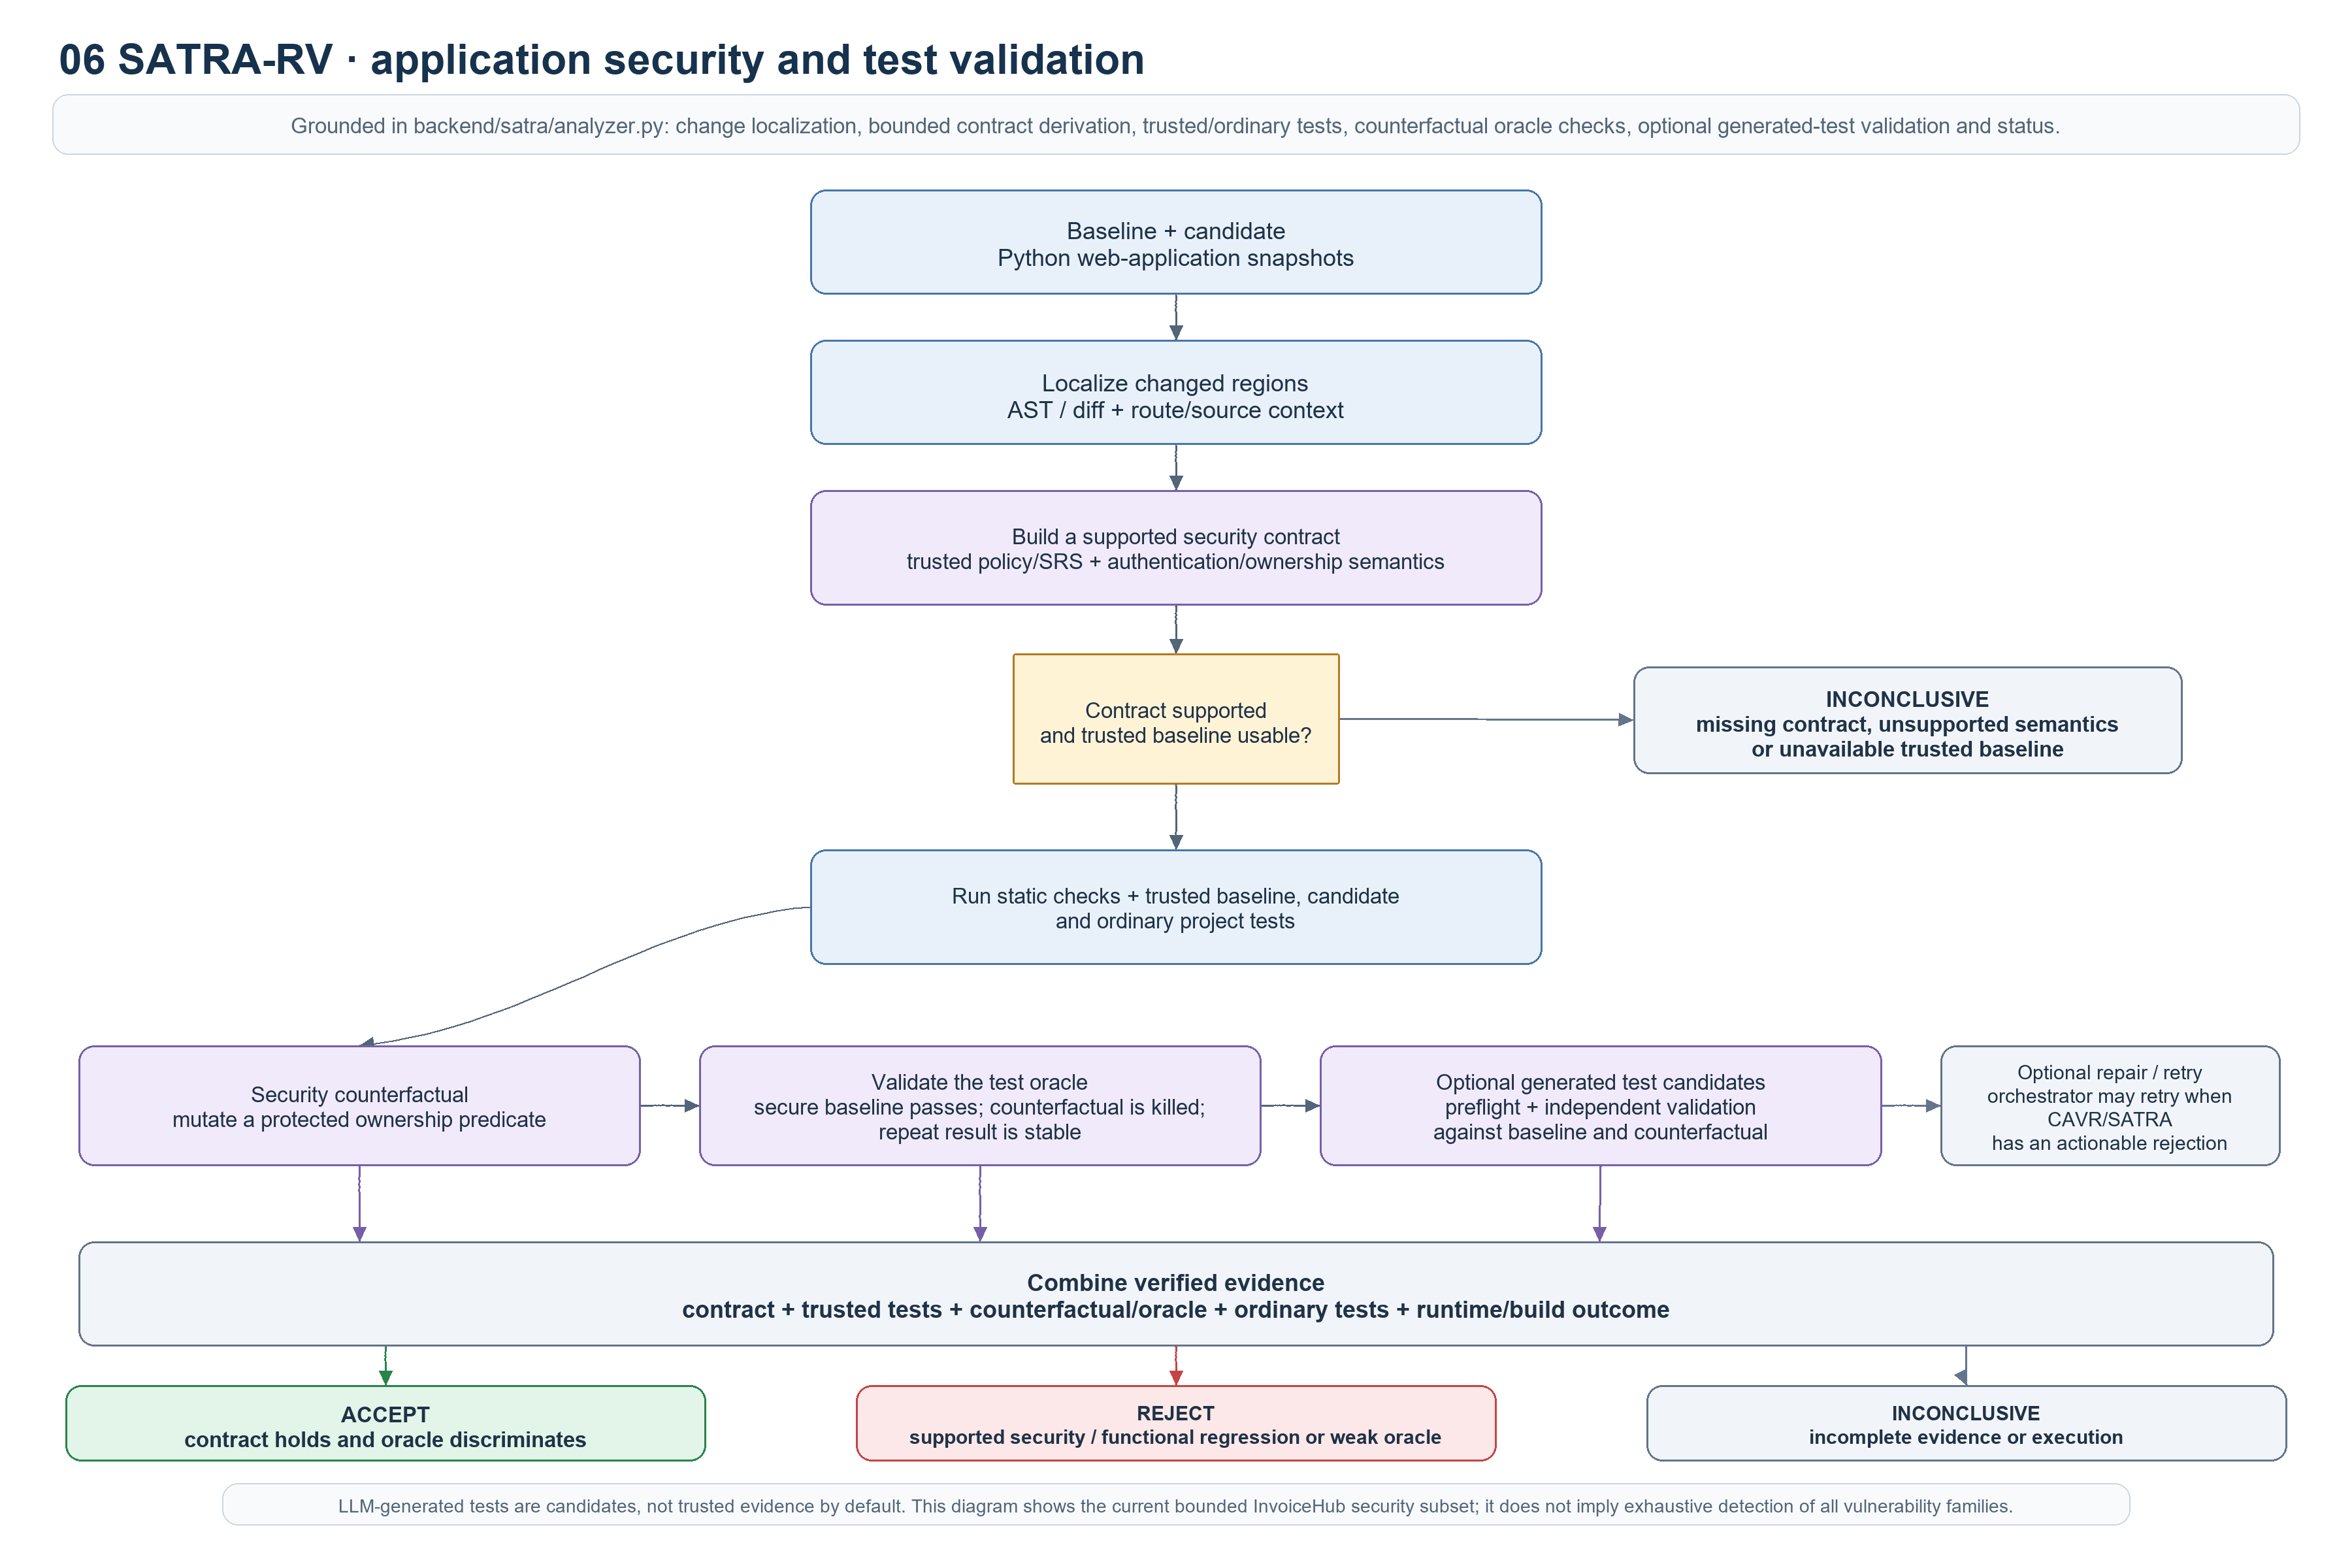
\includegraphics[width=\textheight,height=0.78\textwidth,keepaspectratio]{figures/asent/satra-assurance-flow.png}
\caption{SATRA-RV analysis path from paired source snapshots to an evidence-based result. The diagram is rendered from page 06 of the editable diagrams.net source; generated test candidates are untrusted until validated.}
\label{fig:satra-assurance-flow}
\end{figure}

\begin{figure}[htbp]
\centering
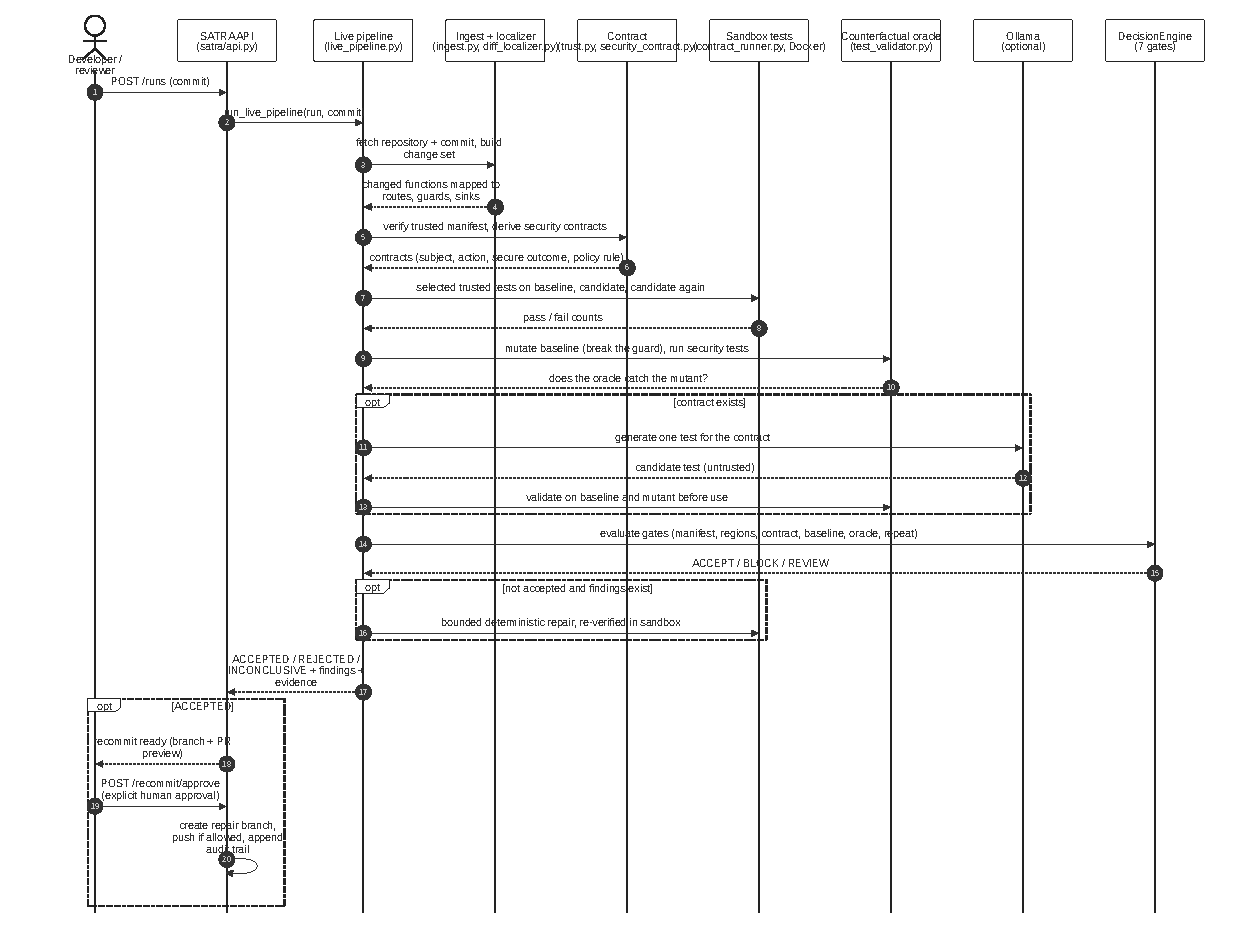
\includegraphics[width=\textwidth]{figures/diagrams/satra-sequence.pdf}
\caption{Sequence of a SATRA-RV live run (\texttt{backend/satra/live\_pipeline.py}) from commit ingestion to the decision and the human-approved recommit.}
\label{fig:satra-sequence}
\end{figure}

\begin{figure}[htbp]
\centering
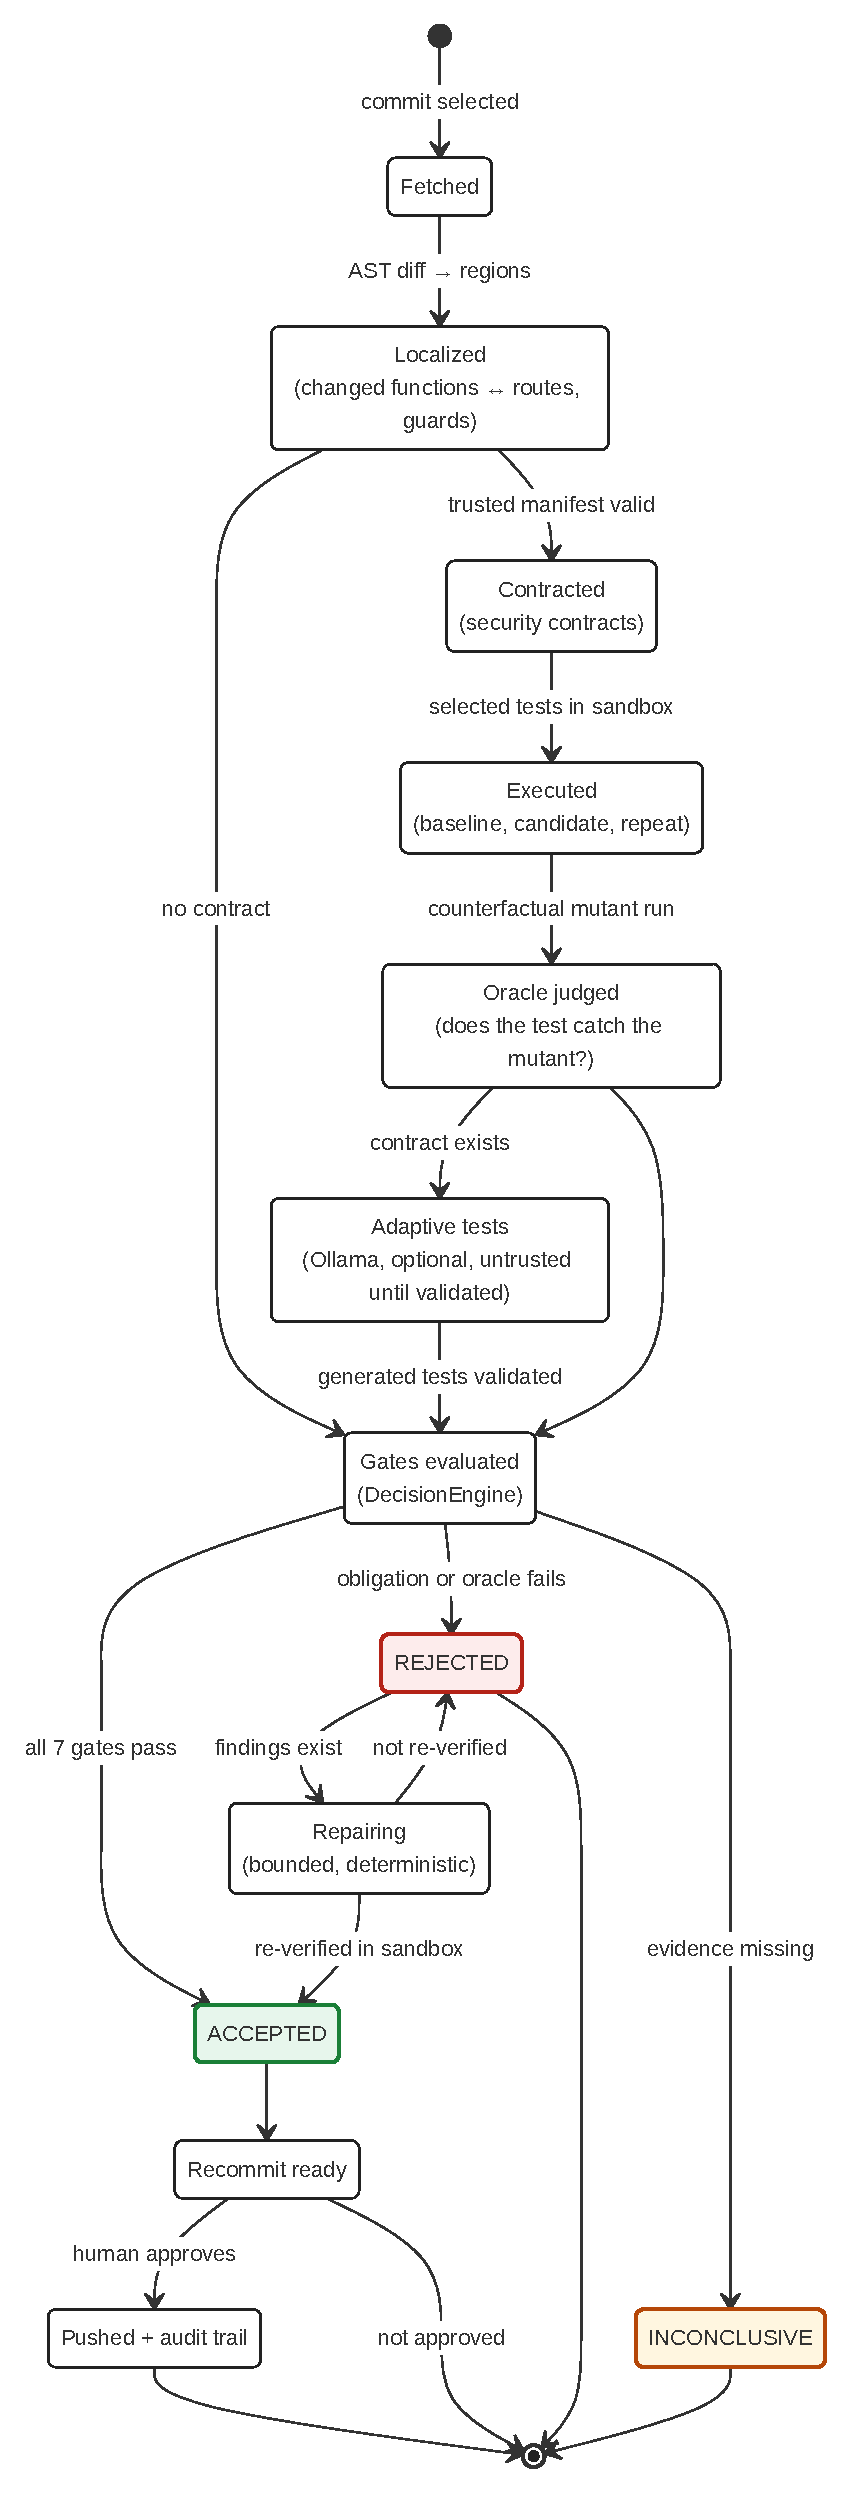
\includegraphics[height=0.8\textheight]{figures/diagrams/satra-state.pdf}
\caption{States of a SATRA-RV run. A repair is only accepted after re-verification in the sandbox, and a recommit is only pushed after explicit human approval.}
\label{fig:satra-state}
\end{figure}

Figures~\ref{fig:satra-sequence} and~\ref{fig:satra-state} show how SATRA-RV judges an application-code change. The commit is fetched and its changed functions are mapped to routes, guards and sinks by AST localization. Security contracts are derived only when the trusted manifest is valid, and the selected trusted tests run in the sandbox on the baseline, the candidate and the candidate again. The counterfactual oracle deliberately breaks the guard in a copy of the baseline and checks that the security tests catch it, so a weak test cannot produce a false pass. Tests generated by Ollama are optional and untrusted until they pass the same validation. The decision engine evaluates seven gates and gives \texttt{ACCEPTED}, \texttt{REJECTED} or \texttt{INCONCLUSIVE}; a rejected run with findings may receive a bounded deterministic repair that counts only after re-verification. An accepted repair is offered as a recommit and is pushed only after an explicit human approval, which is recorded in the audit trail.

\subsection{Implemented Features and Components}
\begin{longtable}{p{0.26\textwidth}p{0.65\textwidth}}
\caption{Implemented Features and Components -- supporting table 1}\\
\toprule
\textbf{Component} & \textbf{Implemented responsibility}\\
\midrule
\path{backend/satra/ingest.py} & Validates allowed repository/ref inputs, resolves commits, records the change set, and prepares isolated baseline/candidate worktrees for the dedicated live pipeline.\\
\path{backend/satra/trust.py} and \path{backend/satra/trusted/} & Verifies SHA-256 fingerprints for trusted SRS, policy, pytest configuration, fixtures, and security tests before use.\\
\path{backend/satra/diff_localizer.py}, \path{astscan.py}, \path{security_contract.py} & Localizes changed Python regions and derives a bounded security contract from supported route and trusted-policy semantics.\\
\path{backend/satra/dictionary.py} & Defines nine rule records. Four Tier-1 entries (IDOR, SQL injection, path traversal, and authentication) have trusted executable tests; five additional rules are marked partial and do not have runnable counterfactual tests in this dictionary.\\
\path{backend/satra/analyzer.py}, \path{contract_runner.py}, \path{pytest_runner.py} & The shared SATRA analyzer runs trusted checks on baseline and candidate, ordinary candidate tests, and a controlled ownership counterfactual, then records test results and reasons. The dedicated live pipeline also maps localized security families and selected routes to trusted test families; the runner uses Docker when present, while its bundled-source fallback is not an arbitrary-code sandbox.\\
\path{backend/satra/test_validator.py}, \path{counterfactuals.py} & Preflight checks generated test syntax and vocabulary, evaluate baseline/mutant/repeat outcomes, and classify an assertion failure separately from an infrastructure error.\\
\path{backend/satra/live_pipeline.py}, \path{ollama_adapter.py} & The dedicated live path can request optional local Ollama test candidates and validate them against the contract and counterfactual; unavailable Ollama is reported as skipped. Model output is not authoritative.\\
\path{backend/satra/decision_engine.py}, \path{repair.py}, \path{repair_inline.py} & The dedicated path evaluates its explicit gate set and may propose bounded deterministic repairs; proposed changes are reported only after re-verification.\\
\path{backend/satra/recommit.py}, \path{audit_trail.py} & Prepare a uniquely named local repair branch with audit metadata, require explicit approval/policy checks before recommit, and maintain a tamper-evident local audit record. This does not establish that a repair was pushed to a production repository.\\
\path{backend/satra/api.py}, \path{frontend/src/components/SatraModule.tsx} & Expose the dedicated SATRA API and React interface, including commit selection, diff, live progress, gate matrix, evidence drawer, and approval interaction.\\
\bottomrule
\end{longtable}

\subsection{Algorithms and Technical Decisions}
The deterministic checks start from a baseline/candidate pair rather than treating a green candidate test suite as sufficient. The localizer associates changed syntax with security-relevant functions and routes. A contract is formed only when the configured trusted policy and supported application semantics provide authority. The trusted tests are run against both sides; the candidate is also checked by its ordinary tests. For the ownership rule, SATRA applies a supported AST counterfactual that removes the ownership guard and checks whether the security oracle rejects it. The validator requires a passing secure baseline, a killed counterfactual, and a repeatable result; execution errors are not classified as successful mutant kills.

The shared analyzer and dedicated live pipeline have distinct status policies and integrations. In the shared route, the bounded analyzer reports \texttt{ACCEPT}, \texttt{REJECT}, or \texttt{INCONCLUSIVE}; the ASENT final gate then checks that applicable evidence is current, integrity-valid, and bound to the same candidate snapshot and module input. The dedicated live pipeline additionally exposes its SATRA gate progression and optional local Ollama stage. Neither path treats generated text as proof. SATRA's module result and ASENT's shared result must therefore be reported separately.

The security dictionary is not uniformly executable. Its four full rules are supported by trusted tests, while the command-injection, insecure-deserialization, SSRF, XSS, and CSRF entries are partial/static or template-level records. The implementation and its UI expose this difference rather than claiming complete detection. Requirements and test names are listed in Chapter~4 and the source test inventory at \path{docs/satra/test-inventory.md}.

The later dedicated live-pipeline update at master commits \texttt{e875904} and \texttt{dfd70d4} adds PR-aware test selection in \path{backend/satra/contract_runner.py}. The selector maps localized security-family identifiers to trusted test files, uses a small route-name fallback when no family is selected, and falls back to the full trusted suite when no test is mapped. It emits a per-family selection reason for the UI. This is bounded prioritization over the available rule and route labels, not complete call-graph reachability. Pruned families are marked as pruned in the result and counted separately, but are not actually executed; no dedicated unit test for the selection mapping was found in the current test tree. Current-master CI passed at \texttt{dfd70d4}; the report therefore records the feature and its limits without presenting the earlier PR~\#5 SATRA test count as specific proof of the selector.

\subsection{Programming Style, Tools, and Technologies}
The implementation uses both procedural and object-oriented programming. Most analyzer stages, AST operations, rule loading, and test evaluation are module-level functions. Object-oriented structures are used where state and interfaces are useful, including Pydantic request/data models, the \texttt{DecisionEngine}, the local Ollama client, and API/service helpers. The React UI is implemented with functional components and hooks. It would be inaccurate to describe the project as exclusively object-oriented or exclusively procedural.

The code uses Python, FastAPI, Pydantic, pytest, Python's AST facilities, Git worktrees, Docker/Podman where available, and a React/TypeScript frontend. Ollama is optional and local to the developer environment; it is not required for the deterministic shared analyzer. CI runs Python 3.12 on Ubuntu and explicitly builds/verifies the SATRA sandbox before the Docker-dependent cases.

\subsection{Demonstration Evidence and Limits}
The integrated source was merged through PR~\#5 at exact tested head \texttt{554b6d51ac\allowbreak{}ca29f99c39\allowbreak{}6c30403620\allowbreak{}15ee460262} (merge \texttt{ffe8aa91}). The SATRA CI run \href{https://github.com/SheharyarAli-Dev/Working-POC/actions/runs/38260995764}{38260995764} and Core CI run \href{https://github.com/SheharyarAli-Dev/Working-POC/actions/runs/38260995652}{38260995652} succeeded on that exact head. The SATRA workflow ran its focused suite and four required Docker sandbox checks; Chapter~7 gives the counts and scope. Later commits \texttt{e875904} and \texttt{dfd70d4} update the dedicated live pipeline and UI. They passed current-master CI runs \href{https://github.com/SheharyarAli-Dev/Working-POC/actions/runs/38540057836}{38540057836} and \href{https://github.com/SheharyarAli-Dev/Working-POC/actions/runs/38542552735}{38542552735}. These later runs establish the recorded repository checks on their exact heads; they do not replace the exact-head PR~\#5 SATRA and Docker-specific counts, or establish isolated test coverage for the new selector.

The repository contains a dedicated SATRA frontend and a recorded defense replay, but this report does not treat a replay as a fresh live run. Fresh completed SATRA-specific browser screenshots and independently reviewed run outputs are not present in the report evidence directory. The integrated Run Workflow rehearsals are SABLE-focused and record SATRA as \texttt{INCONCLUSIVE} on the native-Windows host; they demonstrate the shared gate's handling of that status, not a successful SATRA acceptance. No live cloud deployment is claimed. The source design and test report also leave comparative research, independent benchmark validity, and production-scale detection rates as future work.
